\documentclass[12pt]{book}

% set the cover page
\title{MIT 6.034 Artificial Intelligence} 
\author{Prof. Patrick Henry Winston} 
\date{Fall 2010} 

% redefine section# when create a new SECTION
\renewcommand\thesection{\arabic {section}}
\setcounter{secnumdepth}{3}

% set the page style
\usepackage{geometry}
\geometry{a4paper,left=1.5cm,right=1.5cm,top=2.5cm,bottom=2.5cm}
\usepackage{fancyhdr}
\pagestyle{fancy}
\lhead{} 
\chead{} 
\rhead{} 

%set section's fontstyle
\usepackage{titlesec}
\titleformat*{\section}{\LARGE\bfseries}
\titleformat*{\subsection}{\Large\bfseries}
\titleformat*{\subsubsection}{\large\bfseries}

% include corresponding package
\usepackage{indentfirst}
\usepackage{graphicx, enumerate, amsmath, amsfonts, stmaryrd, amssymb}

% insert hyperlink
\usepackage[colorlinks,linkcolor=blue]{hyperref}

\usepackage{algorithmicx}
\usepackage{algpseudocode}
\usepackage[table,xcdraw]{xcolor}
\begin{document}
	% print the title
	\maketitle 
	% print the content page
	\setcounter{tocdepth}{3}
	\tableofcontents
	\newpage


%----------------------------------------------------------------------------------------
%	INTRODUCTION
%----------------------------------------------------------------------------------------
\section{Introduction} 
\subsection{Definition} % Unnumbered section
\indent \textit{Algorithms enabled by constraints exposed by representations that support models targeted at thinking, perception, and action.}\\
\indent Artificial Intelligence is applied through problem solving procedures, methods, techniques and algorithms.
\subsection{Basic Idea}
\subsubsection{Generate-And-Test Algorithm}
\indent Generate-and-test search algorithm is a very simple algorithm that guarantees to find a solution if done systematically and there exists a solution.\\
\newline
\indent \textbf{Algorithms: }\\
\indent\indent 1. Generate a possible solution.\\
\indent\indent 2. Test to see if this is the expected solution.\\
\indent\indent 3. If the solution has been found quit, else go to step 1.\\
\newline
\indent This approach involved building generators with certain properties: not redundant (should not give the same solution twice), they should also be informable (able to select a category and disregard other)
\subsubsection{Rumpelstiltsin Principle}
\indent Being able to name what you’re talking about gives you power over it, to understand and solve problems. Naming things grants power over concepts.
\subsubsection{Simple $\neq$ Trival}
\indent Trivial ideas implies that they are worthless, useless. In AI, the most simple ideas are often the most powerful.
\newpage
%----------------------------------------------------------------------------------------

\section{Reasoning: Goal Trees and Problem Solving} 
\subsection{Question}
$$\int\frac{-5x^4}{(1-x^2)^{\frac{5}{2}}}dx$$
\indent Is the program, which can solve this 
integral problem, in any sense of the word \textbf{INTELLIGENT}?
\subsection{Model}
\subsubsection{Problem Rediction or AND-OR Tree or Goal Tree}
An and–or tree is a graphical representation of the reduction of problems (or goals) to conjunctions and disjunctions of subproblems (or subgoals).
\begin{figure}[ht]
	\centering
	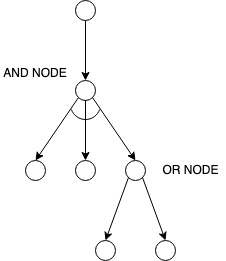
\includegraphics[scale=0.6]{Figure/Figure2_1.png}
	\caption{AND-OR Tree}
\end{figure}
\subsubsection{Architecture}
\begin{figure}[ht]
	\centering
	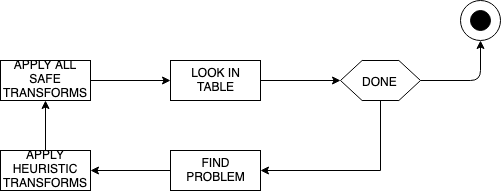
\includegraphics[scale=0.7]{Figure/Figure2_2.png}
	\caption{Problem Solving Architecture}
\end{figure}
\subsection{Transformation}
\subsubsection{Safe Transformation}
\begin{enumerate}
	\item $\int -f(x)dx=-\int f(x)dx$
	\item $\int cf(x)dx=c\int f(x)dx$
	\item $\int \sum f_i(x)dx=\sum \int f_i(x)dx$
	\item $\int \frac{P(x)}{Q(x)}\rightarrow DIVIDE$
\end{enumerate}
 
\subsubsection{Heuristic Transformation}
\begin{enumerate}[A]
 	\item 
 	$
 	f(\sin x, \cos x, \tan x, \cot x, \sec x, \csc x)\rightarrow g_1(\sin x, \cos x)\,or\,g_2(\tan x, \cot x)\,or\,g_3(\sec x, \csc x)$
 	\item 
 	$\int f(\tan x)dx =\int \frac{f(y)}{1+y^2}dy$
 	\item
	$\left\{\begin{array}{l}
	{1-x^2\rightarrow x=\sin y}  \\ {1+x^2\rightarrow x=\tan y}\end{array}\right.$
\end{enumerate}

\subsubsection{Procedure}
\begin{equation*}
\begin{aligned}
\int \frac{-5 x^{4}}{\left(1-x^{2}\right)^{\frac{5}{2}}} d x& \stackrel{1}\longrightarrow \int \frac{5 x^{4}}{\left(1-x^{2}\right)^{\frac{5}{2}}} d x \\
&\stackrel{2}\longrightarrow \int \frac{x^{4}}{\left(1-x^{2}\right)^{\frac{5}{2}}} d x\\
&\stackrel{C}\longrightarrow \int \frac{\sin^4 y}{\cos ^4 y} d y\\
&\stackrel{A}\longrightarrow\left\{\begin{array}{l}
{\int \frac{1}{\cot ^4 s}dx}  \\ {\int \tan ^4 s dx\,\,\,(Choose)}\end{array}\right.\\
&\stackrel{B}\longrightarrow\int\frac{y^4}{1+y^2} d y\\
&\stackrel{4}\longrightarrow \int y^2-1+\frac{1}{1+y^2} d y\\
&\stackrel{3}\longrightarrow\int y^2 dy+\int -1 dy+\int \frac{1}{1+y^2} dy\\
\end{aligned}
\end{equation*}
$$\int -1 dy \stackrel{1}\longrightarrow \int dy\,\,\,and\,\,\,\int \frac{1}{1+y^2} dy\stackrel{C}\longrightarrow \int dz$$
\subsection{Reflection}
KNOWLEDGE ABOUT KNOWLEDGE IS POWER.\\
\indent When we understand how something works, intelligence seems to vanish
\subsection{Questions about the nature of knowledge}
\begin{enumerate}
	\item WHAT kind of knowledge is involved?
	\item HOW is the knowledge represented?
	\item HOW is it used?
	\item HOW much knowledge is required?\\
	Table of integrals: 26 elements.\\
	Safe transformations: 12.\\
	Heuristic transformations: 12.\\
	Then, the integral program is done by \textbf{JAMES SLAGLE} 
	\item WHAT exactly?
\end{enumerate}
\newpage
%----------------------------------------------------------------------------------------

\section{Reasoning: Goal Trees and Rule-Based Expert Systems}
\subsection{Goal Centered Programming}
\subsubsection{Goal}
\begin{figure}[ht]
	\centering
	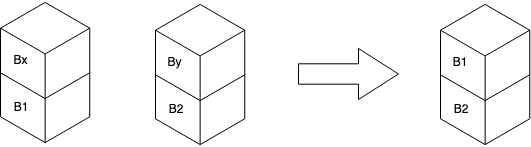
\includegraphics[scale=0.8]{Figure/Figure3_1.png}
	\caption{Put $B_1$ on $B_2$}
\end{figure}
\subsubsection{Function}
\begin{figure}[ht]
	\centering
	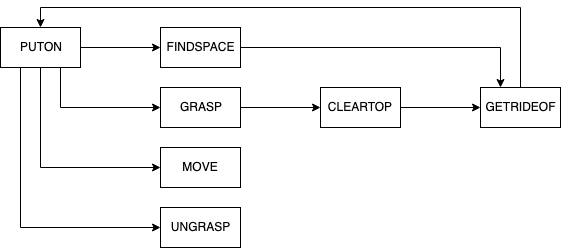
\includegraphics[scale=0.8]{Figure/Figure3_2.png}
	\caption{Related functions}
\end{figure}
\newpage
\subsubsection{Procedure}
\begin{figure}[ht]
	\centering
	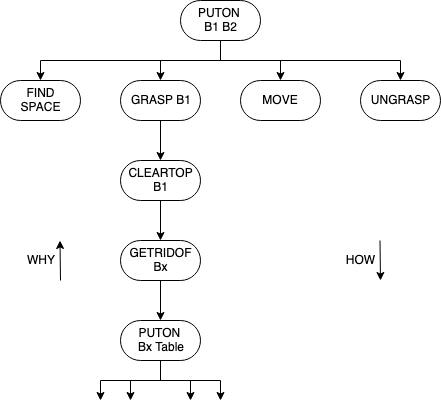
\includegraphics[scale=0.55]{Figure/Figure3_3.png}
	\caption{Related functions}
\end{figure}
\indent For achieve their \textbf{GOALS}, the program leaves a \textbf{TRACE}, which is a \textbf{GOAL TREE}.\\ \indent Then the program can answer questions about its own behavior as long as it builds an and/or tree.\\
\indent Simon's ant: The complexity of the behavior is the max of the complexity of program and the complexity of environment.
\subsection{Rule-Based Expert System}
\begin{figure}[ht]
	\centering
	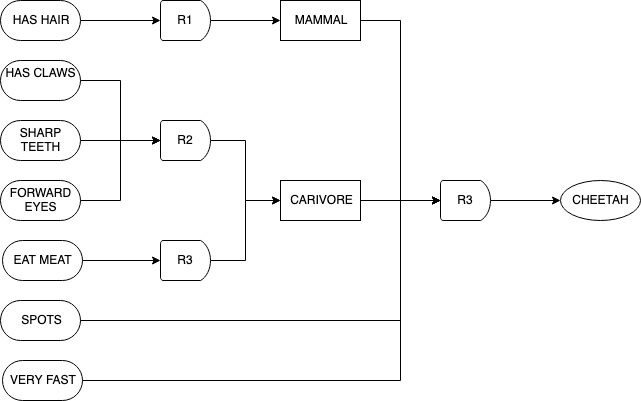
\includegraphics[scale=0.55]{Figure/Figure3_4.png}
	\caption{Forward Chaining Rule-Based Expert System}
\end{figure}
\newpage
%----------------------------------------------------------------------------------------

\section{Search: Depth-First, Hill Climbing, Beam}
\subsection{Question}
\indent Find a path from $S$ to $G$.
\begin{figure}[ht]
	\centering
	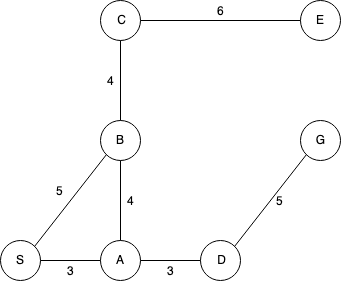
\includegraphics[scale=0.8]{Figure/Figure4_1.png}
	\caption{Map}
\end{figure}
\indent 

\subsection{British Museum Approach--find every possible path}
\begin{figure}[ht]
	\centering
	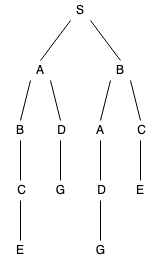
\includegraphics[scale=0.8]{Figure/Figure4_2.png}
	\caption{British Museum Algorithm}
\end{figure}

\subsection{Depth First Search/Breadth First Search}
\indent \indent \indent \textbf{e,g: Depth First Search}\\
\indent \indent \indent \indent (S, A) (S, B)\\
\indent \indent \indent \indent (S, A, B) (S, A, D) (S, B)\\
\indent \indent \indent \indent (S, A, B, C) (S, A, D) (S, B)\\
\indent \indent \indent \indent (S, A, B, C, E) (S, A, D) (S, B)\\
\indent \indent \indent \indent (S, A, D, G) (S, B)

\subsection{Hill Climbing}
\indent just like depth first search instead of using lexical order to break ties, we're going to break ties according to which node is closer to the goal.\\
\newline
\indent \textbf{PROBLEM}
\begin{enumerate}
	\item Local
	\item Telephone Pole Problem
	\item Ridge
\end{enumerate}
\begin{figure}[ht]
	\centering
	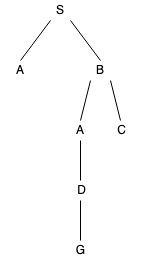
\includegraphics[scale=1]{Figure/Figure4_3.png}
	\caption{Hill Climbing}
\end{figure}
\newpage
\subsection{Beam Search}
\indent complement, addition of and informing heuristic to breadth first search. Limit the number of paths to be considered at any level to some small fixed number.\\
\begin{figure}[ht]
	\centering
	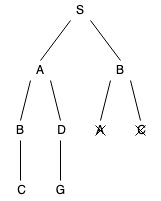
\includegraphics[scale=0.8]{Figure/Figure4_4.png}
	\caption{Beam Search (w=2)}
\end{figure}

\subsection{Procedure}
\begin{figure}[ht]
	\centering
	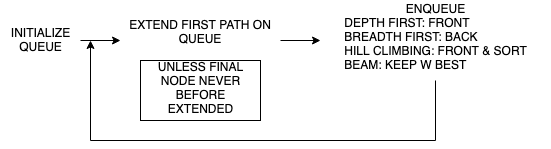
\includegraphics[scale=0.8]{Figure/Figure4_5.png}
	\caption{Procedure}
\end{figure}
\subsection{Property}
\begin{table}[ht]
	\centering
	\begin{tabular}{|c|c|c|c|}
		\hline
		Method         & BACKTRACKING & USE ENQEUE LIST & INFORMED \\ \hline
		BRITISH MUSEUM & X            & X               & X        \\ \hline
		DEPTH FIRST    & V            & V               & X        \\ \hline
		BREADTH FIRST  & X            & V               & X        \\ \hline
		HILL CLIMBING  & V            & V               & V        \\ \hline
		BEAM           & V            & V               & V        \\ \hline
	\end{tabular}
\end{table}
\newpage
\section{Search: Optimal, Branch and Bound, A*}
\subsection{Question: find the best path}
\begin{figure}[ht]
	\centering
	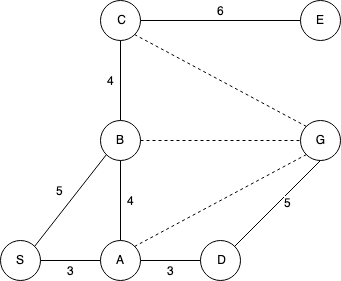
\includegraphics[scale=0.8]{Figure/Figure5_1.png}
	\caption{Map with actual distance \& airline distance}
\end{figure}
\subsection{Branch \& Bound}
\begin{figure}[ht]
	\centering
	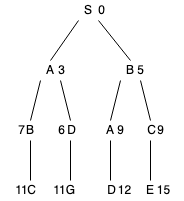
\includegraphics[scale=1]{Figure/Figure5_2.png}
	\caption{Branch \& Bound}
\end{figure}
\newpage
\subsection{with Extended List}
\begin{figure}[ht]
	\centering
	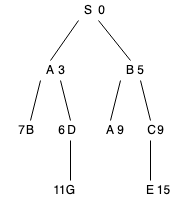
\includegraphics[scale=1]{Figure/Figure5_3.png}
	\caption{Branch \& Bound + Admissible Heuristic}
\end{figure}
\subsection{with Admissible Heuristic}
\begin{figure}[ht]
	\centering
	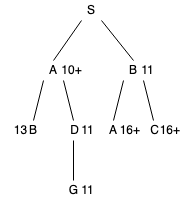
\includegraphics[scale=1]{Figure/Figure5_4.png}
	\caption{Branch \& Bound + Admissible Heuristic}
\end{figure}
\newpage
\subsection{A*}
\begin{figure}[ht]
	\centering
	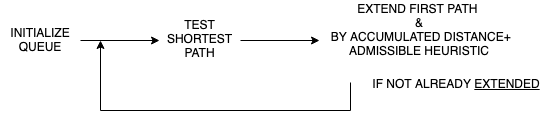
\includegraphics[scale=1]{Figure/Figure5_5.png}
	\caption{Flow Chart}
\end{figure}
\indent\textbf{ADMISSIBLE:} $H(X, G) \leq D(X, G)$\\
\indent\textbf{CONSISTENCE:} $|H(X, G)-H(Y,G)) \leq D(X, Y)$\\
\indent 'Extended' in this part is the pure pass through. Not same as \textbf{Dijkstra’s Algorithm}, so \textbf{A*} may fail at \textbf{non-Euclidean} arrangements
\newpage

\section{Search: Games, Minimax, and Alpha-Beta}
\subsection{Ways to Play}
\begin{enumerate}
	\item \textbf{Analysis} + \textbf{Strategy} + \textbf{Tactics} $\rightarrow$ \textbf{Move}
	\item \textbf{If} $\cdot$ \textbf{Then} Rules
	\item Look Ahead + Evaluate
	\begin{equation*}
	\begin{aligned}
	S=&g(f_1, f_2, \cdots, f_n)\\
	=&c_1f_1+c_2f_2+\cdots+c_nf_n
	\end{aligned}
	\end{equation*}
	\item \textbf{British Museum Algorithm}
	\item *Look Ahead as far as possible 
\end{enumerate}
\subsection{Minimax Algorithm}
\indent Minimax is a kind of backtracking algorithm that is used in decision making and game theory to find the optimal move for a player.\\
\indent In Minimax the two players are called maximizer and minimizer. The maximizer tries to get the highest score possible while the minimizer tries to do the opposite and get the lowest score possible.\\
\indent Every board state has a value associated with it. In a given state if the maximizer has upper hand then, the score of the board will tend to be some positive value. If the minimizer has the upper hand in that board state then it will tend to be some negative value. The values of the board are calculated by some heuristics which are unique for every type of game.
\begin{figure}[ht]
	\centering
	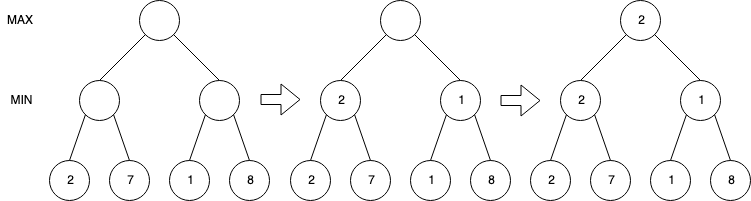
\includegraphics[scale=0.65]{Figure/Figure6_1.png}
	\caption{Minimax Algorithm}
\end{figure}
\subsection{Alpha-Beta Pruning}
\indent Alpha-Beta pruning is not actually a new algorithm, rather an optimization technique for minimax algorithm. It cuts off branches in the game tree which need not be searched because there already exists a better move available.\\
\indent \textbf{Alpha} is the best value that the maximizer currently can guarantee at that level or above.\\
\indent \textbf{Beta} is the best value that the minimizer currently can guarantee at that level or above.
\newpage
Example 1 
\begin{figure}[ht]
		\centering
		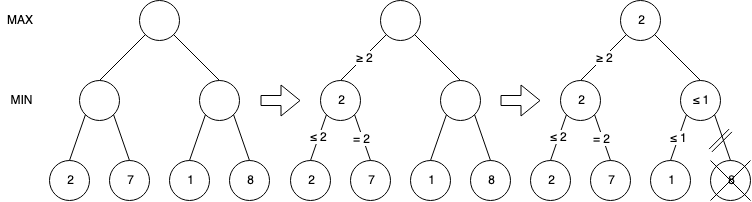
\includegraphics[scale=0.65]{Figure/Figure6_2.png}
		\caption{Alpha-Beta Pruning Algorithm}
	\end{figure}
\newline
\indent Example 2 
\begin{figure}[ht]
	\centering
	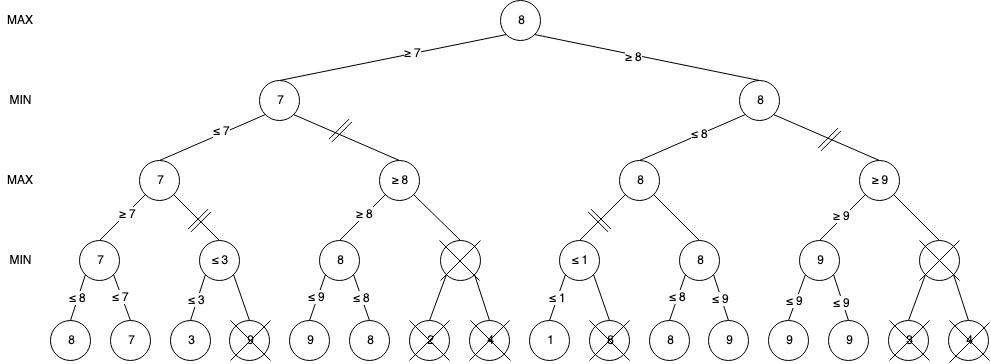
\includegraphics[scale=0.5]{Figure/Figure6_3.png}
	\caption{Alpha-Beta Pruning Algorithm}
\end{figure}

\subsection{Progressive Deepening--Anytime Algorithm}
Start from the very first level,give an insurance policy for every level we try to calculate
$$C=1+b+\cdots+b^{d-1} = \frac{1-b^d}{1-b}=\frac{b^d-1}{b-1}\approx b^{d-1}$$

\subsection{Deep Blue}
DEEP BLUE =   Minimax + $\alpha - \beta$ + Progressive Deepening + Parallel Computing + Opening Book + Special-purpose Stuff for the End Game + \textbf{Uneven Tree Development}
\newpage

\section{Constraints: Interpreting Line Drawings}
\indent \textbf{Object}: Determine how many objects are in a line drawing?
\begin{figure}[ht]
	\centering
	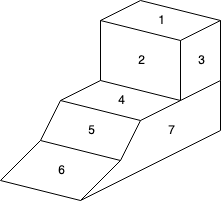
\includegraphics[scale=0.6]{Figure/Figure7_1.png}
	\caption{Line Drawing}
\end{figure}
\subsection{Guzman's Solution}
\textbf{Two perspectives}
\begin{figure}[htbp]
	\centering
	\begin{minipage}[t]{0.48\textwidth}
		\centering
		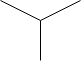
\includegraphics[]{Figure/Figure7_2.png}
		\caption{Fork type junction}
	\end{minipage}
	\begin{minipage}[t]{0.48\textwidth}
		\centering
		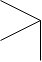
\includegraphics[]{Figure/Figure7_3.png}
		\caption{Arrow type junction}
	\end{minipage}
\end{figure}
\begin{enumerate}
	\item Fork type junctions: three pairs of faces seem to belong to the same object. 
	\item Arrow type junctions: faces on either side of she shaft belong to the same object.
\end{enumerate}
\indent \indent \textbf{Transform the line drawing to a GRAPH}
\begin{figure}[htbp]
	\centering
	\begin{minipage}[t]{0.32\textwidth}
	\centering
	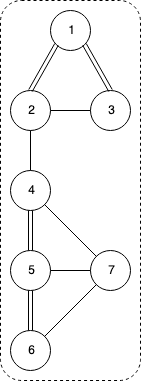
\includegraphics[height=6.4cm]{Figure/Figure7_4.png}
	\caption{1 LINK}
	\end{minipage}
	\begin{minipage}[t]{0.32\textwidth}
		\centering
		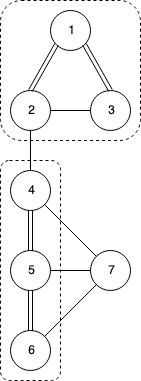
\includegraphics[height=6.4cm]{Figure/Figure7_5.png}
		\caption{2 LINK}
	\end{minipage}
	\begin{minipage}[t]{0.32\textwidth}
	\centering
	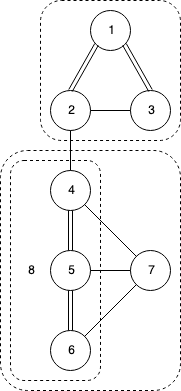
\includegraphics[height=6.4cm]{Figure/Figure7_6.png}
	\caption{2 LINK*}
	\end{minipage}
\end{figure}
\subsection{Dave Huffman's Solution}
\textbf{Construct a mathematical model (Three Assumptions)}
\begin{enumerate}
	\item General Position
	\begin{figure}[htbp]
		\centering
		\begin{minipage}[t]{0.48\textwidth}
			\centering
			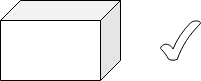
\includegraphics[]{Figure/Figure7_7.png}
			\caption{Nice case}
		\end{minipage}
		\begin{minipage}[t]{0.48\textwidth}
			\centering
			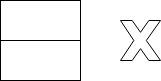
\includegraphics[]{Figure/Figure7_8.png}
			\caption{Weird case}
		\end{minipage}
	\end{figure}
	\item Trihedral:  all vertexes out there are going to be formed from three planes.
	\item Four kinds of symbols
		\begin{figure}[htbp]
		\centering
		\begin{minipage}[t]{0.23\textwidth}
			\centering
			
\includegraphics[]{Figure/Figure7_9.png}
			\caption{Convex}
		\end{minipage}
		\begin{minipage}[t]{0.23\textwidth}
			\centering
			
\includegraphics[]{Figure/Figure7_10.png}
			\caption{Concave}
		\end{minipage}
		\begin{minipage}[t]{0.23\textwidth}
			\centering
			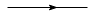
\includegraphics[]{Figure/Figure7_11.png}
			\caption{Boundary}
		\end{minipage}
		\begin{minipage}[t]{0.23\textwidth}
			\centering
			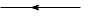
\includegraphics[]{Figure/Figure7_12.png}
			\caption{Boundary}
		\end{minipage}
	\end{figure}
	\newline
	\textbf{*Boundary}: which side you would see the object if you walk along the direction of this arrow
\end{enumerate}
\indent \indent \textbf{All possible ways that junctions can have line labels arranged around them}
\begin{figure}[ht]
	\centering
	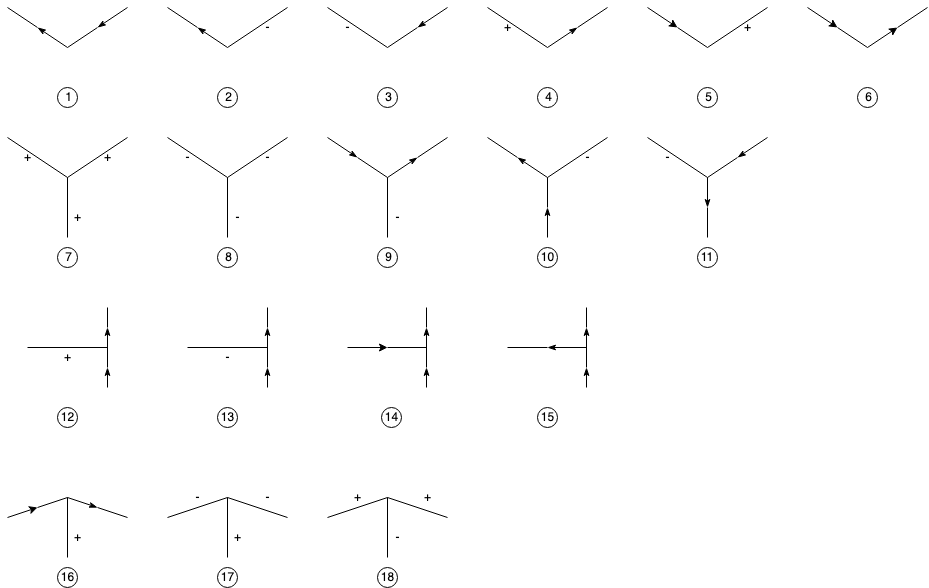
\includegraphics[scale=0.49]{Figure/Figure7_13.png}
	\caption{All kinds of junctions}
\end{figure}
\subsection{David Waltz's Solution}
\textbf{+ CRACKS}\\
\indent \textbf{+ SHADOWS}\\
\indent \textbf{+ NON-TRIHEDRAL VERTEXES}\\
\indent \textbf{+ LIGHT}\\
\indent Then, $4$ labels $\Longrightarrow$ $50^+$ labels, $18$ junctions $\Longrightarrow$ $1000's$ junctions.\newline \newline
\textbf{Waltz's Algorithms} (use Huffman's set to demonstrate \href{https://www.youtube.com/watch?v=l-tzjenXrvI#t=38m16s}{Waltz's algorithm})
\newpage
\section{Constraints: Search, Domain Reduction}
\textbf{Object: Graph Coloring}
\subsection{Term}
\begin{enumerate}
	\item \textbf{Variable} $v$: something that can have assignment
	\item \textbf{Value} $x$: something can be an assignment
	\item \textbf{Domain} $D$: bag of value
	\item \textbf{Constrain} C: limit on variable values
\end{enumerate}
\subsection{Procedure--Domain Reduction Algorithm}
\begin{algorithmic}
	\For {each DFS assignment}
	\For {each variable $v_i$ considered}
	\For {each $x_i$ in $D_i$}
	\For {each constraint $C(x_i,x_j)$ where $x_j\in D_j$}
	\If {$\nexists$ $x_j$ $\ni$ $C(x_i,x_j)$ satisfied}
	\State {remove $x_i$ from $D_i$}
	\EndIf
	\If {$D_i$ is empty}
	\State {backup}
	\EndIf
	\EndFor
	\EndFor
	\EndFor
	\EndFor
\end{algorithmic}
\subsection{Consider}
\begin{enumerate}
	\item Nothing
	\item Assignment
	\item Check Neighbors
	\item \textbf{Propagate} Checking $v$ with $D$ Reduced to $1$ Value  
	\item \textbf{Propagate} Checking through $v$ with Reduced $D$   
	\item Everything
\end{enumerate}
\newpage

\section{Constraints: Visual Object Recognition}
\subsection{David Marr's idea--JUST A IDEA}
\textbf{IDEA}: Based on the idea that you start off by looking at edges and you end up in several steps of transformation, producing something that you can look up in a library of descriptions.\\
\begin{figure}[ht]
	\centering
	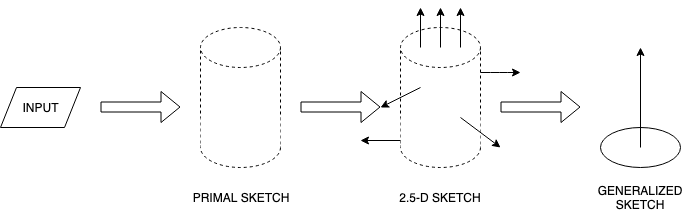
\includegraphics[scale=0.6]{Figure/Figure9_1.png}
	\caption{Marr's idea}
\end{figure}
\begin{enumerate}
	\item Input from camera
	\item Form this edge based description of what's out there in the world
	\item Decorate the primal sketch with some vectors, some surface normals, showing where the faces on the object are oriented
	\item Transform this 2.5 dimensional sketch to generalized sketch (function+direction)
	\item Match against the library of such descriptions, and results in recognition
\end{enumerate}
\subsection{Shimon Ullman--Alignment Theory}
\textbf{IDEA}: Assume we have a transparent object where all the vertexes are visible, and neglect the effect of perspectives, then we can reconstruct any view of that object.\\
\indent $\Theta_A$, $\Theta_B$ and $\Theta_U$ are corresponding angles between $\vec S$ and $\vec A$, $\vec B$, $\vec U$. If we only consider 2D rotation, we need two picture as follows.\\
\begin{figure}[ht]
	\centering
	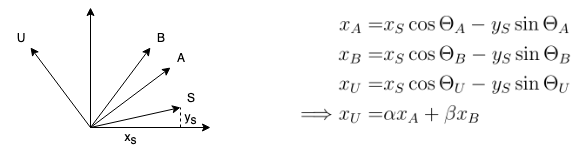
\includegraphics[scale=0.6]{Figure/Figure9_2.png}
	\caption{Example}
\end{figure}
\newline
\indent If include translation element, we need add a constant item $\tau$.  
\subsection{Correlation  Theory}
$$\max_{X,Y}\int f(x,y)g(x-X,y-Y)$$
\indent To some extends, it's like convolution. However, this course was opened in 2010, but CNN was presented in 2012, so there is not much explanation here.
\newpage

\section{Introduction to Learning, Nearest Neighbors}
\subsection{Types of Learning}
\begin{figure}[ht]
	\centering
	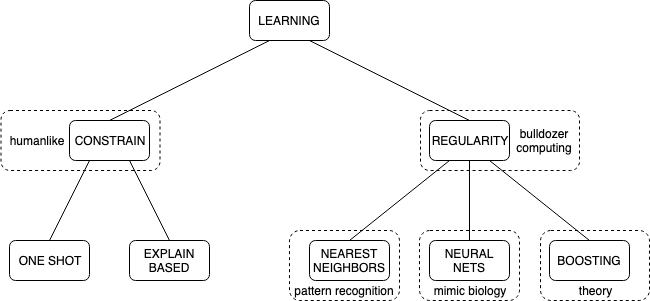
\includegraphics[scale=0.7]{Figure/Figure10_1.png}
	\caption{Learning types}
\end{figure}
\subsection{Mechanism of Pattern Recognition}
\begin{figure}[ht]
	\centering
	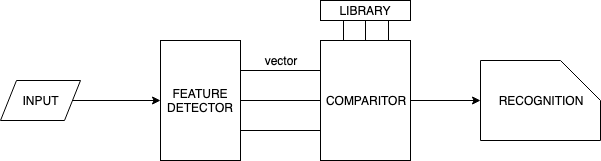
\includegraphics[scale=0.7]{Figure/Figure10_2.png}
	\caption{Mechanism of Pattern Recognition}
\end{figure}
\href{https://www.youtube.com/watch?time_continue=4&v=09mb78oiPkA#t=9m00s}{Use Different Distance Metric to Generate Decision Boundary}
\subsection{Learning}
\href{https://www.youtube.com/watch?time_continue=4&v=09mb78oiPkA#t=24m18s}{Why LEARNING?}
\newpage
\section{Learning: Identification Trees, Disorder}
\subsection{Target}
Use data to build a recognition mechanism
\begin{table}[ht]
	\centering
	\begin{tabular}{|c|c|c|c|c|}
		\hline
		\rowcolor[HTML]{C0C0C0} 
		{\color[HTML]{000000} \textbf{Vampire}} & {\color[HTML]{000000} \textbf{Shadow}} & {\color[HTML]{000000} \textbf{Garlic}} & {\color[HTML]{000000} \textbf{Complexion}} & {\color[HTML]{000000} \textbf{Accent}} \\ \hline
		{\color[HTML]{000000} \textbf{No}}      & {\color[HTML]{000000} ?}               & {\color[HTML]{000000} Yes}             & {\color[HTML]{000000} PALE}                & {\color[HTML]{000000} None}            \\ \hline
		\rowcolor[HTML]{FFFFFF} 
		{\color[HTML]{000000} \textbf{No}}      & {\color[HTML]{000000} Yes}             & {\color[HTML]{000000} Yes}             & {\color[HTML]{000000} Ruddy}               & {\color[HTML]{000000} None}            \\ \hline
		{\color[HTML]{000000} \textbf{Yes}}     & {\color[HTML]{000000} ?}               & {\color[HTML]{000000} No}              & {\color[HTML]{000000} Ruddy}               & {\color[HTML]{000000} None}            \\ \hline
		{\color[HTML]{000000} \textbf{Yes}}     & {\color[HTML]{000000} No}              & {\color[HTML]{000000} No}              & {\color[HTML]{000000} Average}             & {\color[HTML]{000000} Heavy}           \\ \hline
		{\color[HTML]{000000} \textbf{Yes}}     & {\color[HTML]{000000} ?}               & {\color[HTML]{000000} No}              & {\color[HTML]{000000} Average}             & {\color[HTML]{000000} Odd}             \\ \hline
		{\color[HTML]{000000} \textbf{No}}      & {\color[HTML]{000000} Yes}             & {\color[HTML]{000000} No}              & {\color[HTML]{000000} Pale}                & {\color[HTML]{000000} Heavy}           \\ \hline
		{\color[HTML]{000000} \textbf{No}}      & {\color[HTML]{000000} Yes}             & {\color[HTML]{000000} No}              & {\color[HTML]{000000} Average}             & {\color[HTML]{000000} Heavy}           \\ \hline
		{\color[HTML]{000000} \textbf{No}}      & {\color[HTML]{000000} ?}               & {\color[HTML]{000000} Yes}             & {\color[HTML]{000000} Ruddy}               & {\color[HTML]{000000} Odd}             \\ \hline
	\end{tabular}
\end{table}
\subsection{Difference between the Dataset of Identification Tree and Nearest Neighbor}
\begin{enumerate}
	\item Some features are non-numeric
	\item Some features don't matter
	\item Some features only some of time
	\item Some tests Cost
	\item *Identification tree is talking in terms of \textbf{tests}, not a \textbf{vector of real values}
\end{enumerate}
\subsection{Procedure——Occam's Razor}
\subsubsection{Naive Strategy}
Based on the number of sample individuals are put into a homogeneous set.
\begin{figure}[ht]
	\centering
	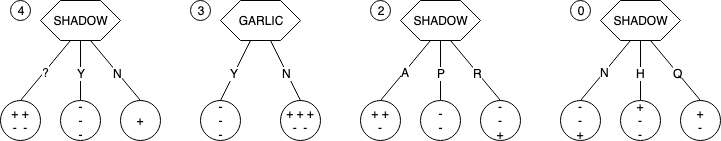
\includegraphics[scale=0.7]{Figure/Figure11_1.png}
	\caption{First test}
\end{figure}
\newpage
\begin{table}[ht]
	\centering
	\begin{tabular}{|c|c|c|c|c|}
		\hline
		\rowcolor[HTML]{C0C0C0} 
		{\color[HTML]{000000} \textbf{Vampire}} & {\color[HTML]{000000} \textbf{Shadow}} & {\color[HTML]{000000} \textbf{Garlic}} & {\color[HTML]{000000} \textbf{Complexion}} & {\color[HTML]{000000} \textbf{Accent}} \\ \hline
		{\color[HTML]{000000} \textbf{No}}      & {\color[HTML]{000000} ?}               & {\color[HTML]{000000} Yes}             & {\color[HTML]{000000} PALE}                & {\color[HTML]{000000} None}            \\ \hline
		\rowcolor[HTML]{000000} 
		{\color[HTML]{000000} \textbf{No}}      & {\color[HTML]{000000} Yes}             & {\color[HTML]{000000} Yes}             & {\color[HTML]{000000} Ruddy}               & {\color[HTML]{000000} None}            \\ \hline
		{\color[HTML]{000000} \textbf{Yes}}     & {\color[HTML]{000000} ?}               & {\color[HTML]{000000} No}              & {\color[HTML]{000000} Ruddy}               & {\color[HTML]{000000} None}            \\ \hline
		\rowcolor[HTML]{000000} 
		{\color[HTML]{000000} \textbf{Yes}}     & {\color[HTML]{000000} No}              & {\color[HTML]{000000} No}              & {\color[HTML]{000000} Average}             & {\color[HTML]{000000} Heavy}           \\ \hline
		{\color[HTML]{000000} \textbf{Yes}}     & {\color[HTML]{000000} ?}               & {\color[HTML]{000000} No}              & {\color[HTML]{000000} Average}             & {\color[HTML]{000000} Odd}             \\ \hline
		\rowcolor[HTML]{000000} 
		{\color[HTML]{000000} \textbf{No}}      & {\color[HTML]{000000} Yes}             & {\color[HTML]{000000} No}              & {\color[HTML]{000000} Pale}                & {\color[HTML]{000000} Heavy}           \\ \hline
		\rowcolor[HTML]{000000} 
		{\color[HTML]{000000} \textbf{No}}      & {\color[HTML]{000000} Yes}             & {\color[HTML]{000000} No}              & {\color[HTML]{000000} Average}             & {\color[HTML]{000000} Heavy}           \\ \hline
		{\color[HTML]{000000} \textbf{No}}      & {\color[HTML]{000000} ?}               & {\color[HTML]{000000} Yes}             & {\color[HTML]{000000} Ruddy}               & {\color[HTML]{000000} Odd}             \\ \hline
	\end{tabular}
\end{table}
\begin{figure}[ht]
	\centering
	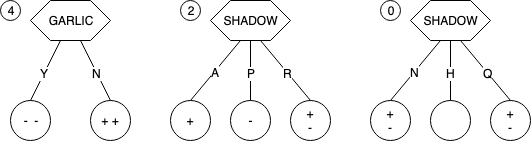
\includegraphics[scale=0.7]{Figure/Figure11_2.png}
	\caption{Second test}
\end{figure}
\indent Then, we can construct a identification tree
\begin{figure}[ht]
	\centering
	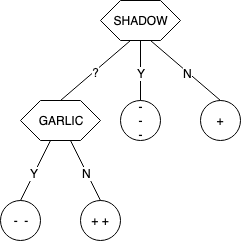
\includegraphics[scale=0.7]{Figure/Figure11_3.png}
	\caption{Identification tree}
\end{figure}
\subsubsection{Large Dataset}
Evaluate the disorder in sets.
$$D(set) = -\frac{P}{T}\log_2\frac{P}{T}-\frac{N}{T}\log_2\frac{N}{T}$$
$$Q(test) = \sum_{sets produced}D(set)\frac{\# of \,\, samples \,\, in \,\, set}{\# of \,\, samples \,\, handled \,\, in \,\, test}$$
\begin{figure}[ht]
	\centering
	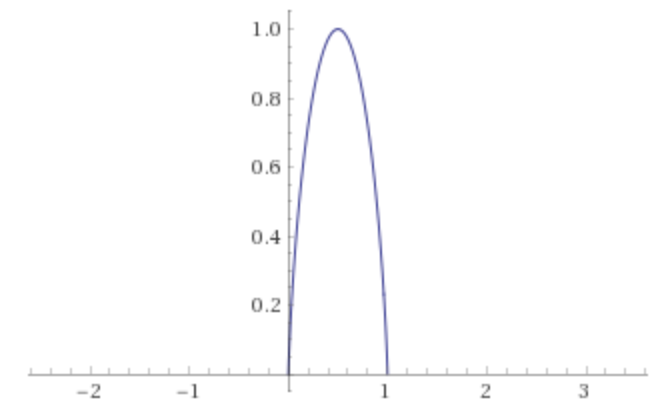
\includegraphics[scale=0.7]{Figure/Figure11_4.png}
	\caption{The relationship between $D(set)$ and $\frac{P}{T}$}
\end{figure}\newline
\indent Then we will get the same answer as shown in Figure 39
\subsection{Decision Boundary}
	\begin{figure}[htbp]
	\centering
	\begin{minipage}[t]{0.48\textwidth}
		\centering
		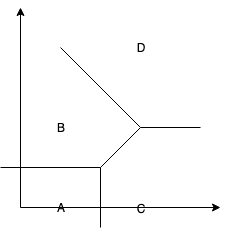
\includegraphics[]{Figure/Figure11_5.png}
		\caption{Nearest neighbors}
	\end{minipage}
	\begin{minipage}[t]{0.48\textwidth}
		\centering
		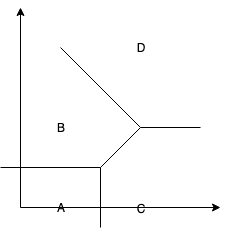
\includegraphics[]{Figure/Figure11_5.png}
		\caption{Identification tree}
	\end{minipage}
\end{figure}
\subsection{Tree to Rule}
\indent Go down each branch to the leaf. Sometimes, we can simplify the description. 
\newpage
\section{Neural Nets}
 \subsection{Model Real Neuron}
 \begin{figure}[ht]
 	\centering
 	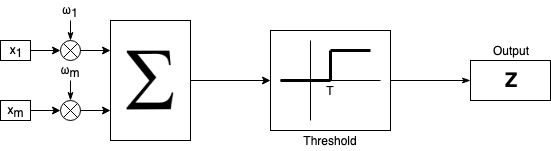
\includegraphics[scale=0.7]{Figure/Figure12_1.png}
 	\caption{Neural Model}
 \end{figure}
\textbf{INCLUDE}
\begin{enumerate}
	\item All or none
	\item Cumulative influence
	\item Synaptic weight
\end{enumerate}
\indent \indent \textbf{EXCLUDE}
\begin{enumerate}
	\item Refractory period
	\item Axonal bifurcation
	\item Time patterns
\end{enumerate}
\subsection{Training}
\begin{figure}[ht]
	\centering
	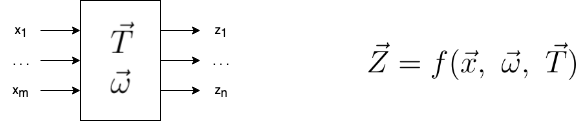
\includegraphics[scale=0.7]{Figure/Figure12_2.png}
	\caption{Neural Model}
\end{figure}
Training a neural net is adjusting these weights and thresholds.
$$Neural\,\,Net\,\,\Longrightarrow\,\,Function\,\,Approximator$$
\indent \textbf{desired}: $\vec{d}=g(\vec{X})$\\
\indent \textbf{performance}: $P=-\frac{1}{2}||\vec{d}-\vec{a}||^2$ (define for mathematical convenient)
\newpage
\subsection{Gradient Descent}
\begin{figure}[ht]
	\centering
	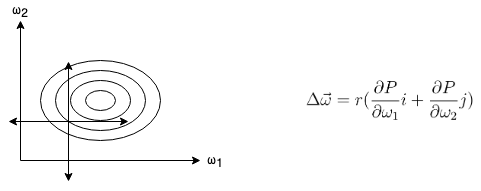
\includegraphics[scale=0.7]{Figure/Figure12_3.png}
	\caption{Gradient Descent}
\end{figure}
\textbf{But we cannot use gradient descent/ascent--Discontinuous for our function.}
\begin{figure}[ht]
	\centering
	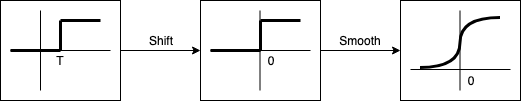
\includegraphics[scale=0.7]{Figure/Figure12_4.png}
	\caption{Change threshold function}
\end{figure}
\subsection{}
\begin{figure}[ht]
	\centering
	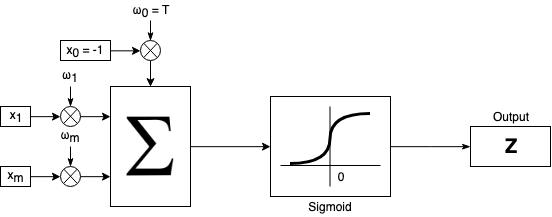
\includegraphics[scale=0.7]{Figure/Figure12_5.png}
	\caption{New Neural Model}
\end{figure}
For sigmoid function $\beta=\frac{1}{1+e^{-\alpha}}$:
\begin{equation*}
\begin{aligned}
	\frac{d\beta}{d\alpha}=&\frac{d}{d\alpha}(1+e^{-\alpha})^{-1}\\
	=&e^{-\alpha}(1+e^{-\alpha})^{-2}\\
	=&\frac{e^{-\alpha}}{1+e^{-\alpha}}\cdot \frac{1}{1+e^{-\alpha}}\\
	=&\beta(1-\beta)
\end{aligned}
\end{equation*}
\newpage
\subsection{Backpropagation Algorithm}
\begin{figure}[ht]
	\centering
	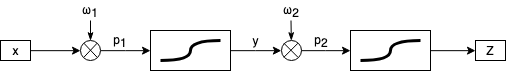
\includegraphics[scale=0.7]{Figure/Figure12_6.png}
	\caption{Sample Neural Net}
\end{figure}
\begin{equation*}
\begin{aligned}
	\frac{\partial P}{\partial \omega_2} = &\frac{\partial P}{\partial z}\cdot \frac{\partial z}{\partial p_2}\cdot \frac{\partial p_2}{\partial \omega_2}\\
	\frac{\partial P}{\partial \omega_1} = &\frac{\partial P}{\partial z}\cdot \frac{\partial z}{\partial p_2}\cdot \frac{\partial p_2}{\partial y}\cdot \frac{\partial y}{\partial p_1}\cdot\frac{\partial p_1}{\partial \omega_1}\\
\end{aligned}
\end{equation*}

\begin{equation*}
\begin{aligned}
	\frac{\partial P}{\partial z}\cdot \frac{\partial z}{\partial p_2}\cdot \frac{\partial p_2}{\partial \omega_2}=&y\cdot z(1-z)\cdot(d-z)\\
	\frac{\partial P}{\partial z}\cdot \frac{\partial z}{\partial p_2}\cdot \frac{\partial p_2}{\partial y}\cdot \frac{\partial y}{\partial p_1}\cdot\frac{\partial p_1}{\partial \omega_1}=&x\cdot y(1-y)\cdot \omega_2\cdot z(1-z)\cdot(d-z)
\end{aligned}
\end{equation*}
\newpage
\section{Learning: Genetic Algorithms}
\begin{figure}[ht]
	\centering
	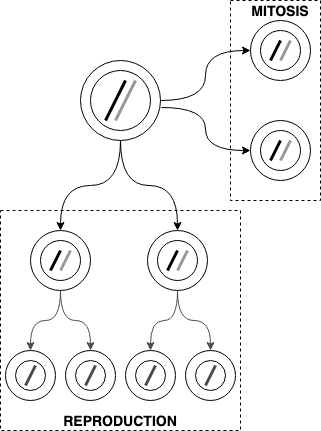
\includegraphics[scale=0.7]{Figure/Figure13_1.png}
	\caption{Genetic Biology}
\end{figure}
\subsection{Imitation (ATCG $\longrightarrow$ 01)}
\begin{figure}[ht]
	\centering
	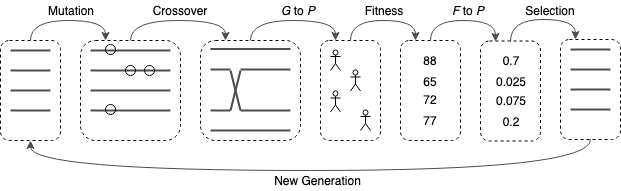
\includegraphics[scale=0.7]{Figure/Figure13_2.png}
	\caption{Genetic Algorithm}
\end{figure}
\noindent\textbf{G}: Genotype\\
\textbf{P}: Phenotype\\
\textbf{F}: Fitness\\
\textbf{P}: Probability
\newpage
\subsection{Mechanism}
\subsubsection{Fitness}
$$P_i = \frac{f_i}{\sum_j f_j}$$
$$f(x,y)=(\sin\omega x)^2(\sin\omega y)^2e^{-\frac{x+y}{\sigma}}$$
\subsubsection{Rank Space}
\begin{equation*}
\begin{aligned}
P_1 = &P_c\\
P_2 = &(1-P_c)P_c\\
\cdots\\
P_{n-1}=&(1-P_c)^{n-2}P_c\\
P_n = & (1-P_c)^{n-1}
\end{aligned}
\end{equation*}
\subsubsection{Diversity}
\begin{figure}[ht]
	\centering
	\includegraphics[scale=0.7]{Figure/Figure13_3.png}
	\caption{Genetic Biology}
\end{figure}
\newpage
\section{Learning: Sparse Spaces, Phonology}
\subsection{Point}
\begin{figure}[ht]
	\centering
	\includegraphics[scale=0.65]{Figure/Figure14_1.png}
	\caption{Learning Process}
\end{figure}
\subsection{Phonological Rules}
\subsubsection{Distinctive features Theory}
\begin{figure}[ht]
	\centering
	\includegraphics[scale=0.65]{Figure/Figure14_2.png}
	\caption{Distinctive features}
\end{figure}
\subsubsection{YIP-SUSSMAN Machine/Learner}
\begin{figure}[ht]
	\centering
	\includegraphics[scale=0.65]{Figure/Figure14_3.png}
	\caption{YIP-SUSSMAN Machine}
\end{figure}
\newpage
\begin{figure}[ht]
	\centering
	\includegraphics[scale=0.6]{Figure/Figure14_4.png}
	\caption{Four distinctive features of "APPLES"}
\end{figure}
If we present this machine with a pair of apples.
\begin{figure}[ht]
	\centering
	\includegraphics[scale=0.65]{Figure/Figure14_5.png}
	\caption{Work flow}
\end{figure}
\begin{enumerate}
	\item The vision apparatus comes in and produces the notation, the concept of 2 apples.
	\item Information flows from that meaning register to the "APPLE" word; information also flows to the register and mark it as plus plural
	\item Information flows from word to register so as to indicate that it's a noun but not a verb; also writes "a", "p", and "l" into the buffer
	\item Left flow of the word
\end{enumerate}
\subsection{Sparse Spaces*(!More information need)}
\begin{enumerate}
	\item COLLECT positive(+) and negative(-) examples
	\item PICK positive(+) seed
	\item GENERALIZE $+\,\longrightarrow *$("*" means "Don't care")
	\item UNTIL we admit or match a negative example
\end{enumerate}
\subsection{Marr's Catechism}
\begin{enumerate}
	\item Specify the problem
	\item Devise a representation
	\item Determine an approach/thought/method
	\item Pick a mechanism/Devise a algorithm
	\item Experiment 
\end{enumerate}
\newpage
\section{Learning: Near Misses, Felicity Conditions}

\newpage
\section{Learning: Support Vector Machines}

\newpage
\section{Learning: Boosting}

\newpage
\section{Representations: Classes, Trajectories, Transitions}

\newpage
\section{Architectures: GPS, SOAR, Subsumption, Society of Mind}

\newpage
\section{Probabilistic Inference I}

\newpage
\section{Probabilistic Inference II}

\newpage
\section{Model Merging, Cross-Modal Coupling, Course Summary}
\end{document}